% python figure_flame2.py --load -m fwd optim eps 

\section{Model and Inversion of Flaming Aurora}\label{sec:flame}
We model two time steps of a flaming auroral event with $E_0\in\lbrace{4.5,1.6\rbrace}$~keV. 
The input differential number flux $\Phi_{top}$ is shown in Fig.~\ref{fig:estflame}(a)(c). 
Fig.~\ref{fig:estflame}(b)(d) show the estimated differential number flux $\hat{\Phi}_{top}$ using the L-BFGS-B algorithm. 
%
\begin{figure}\centering
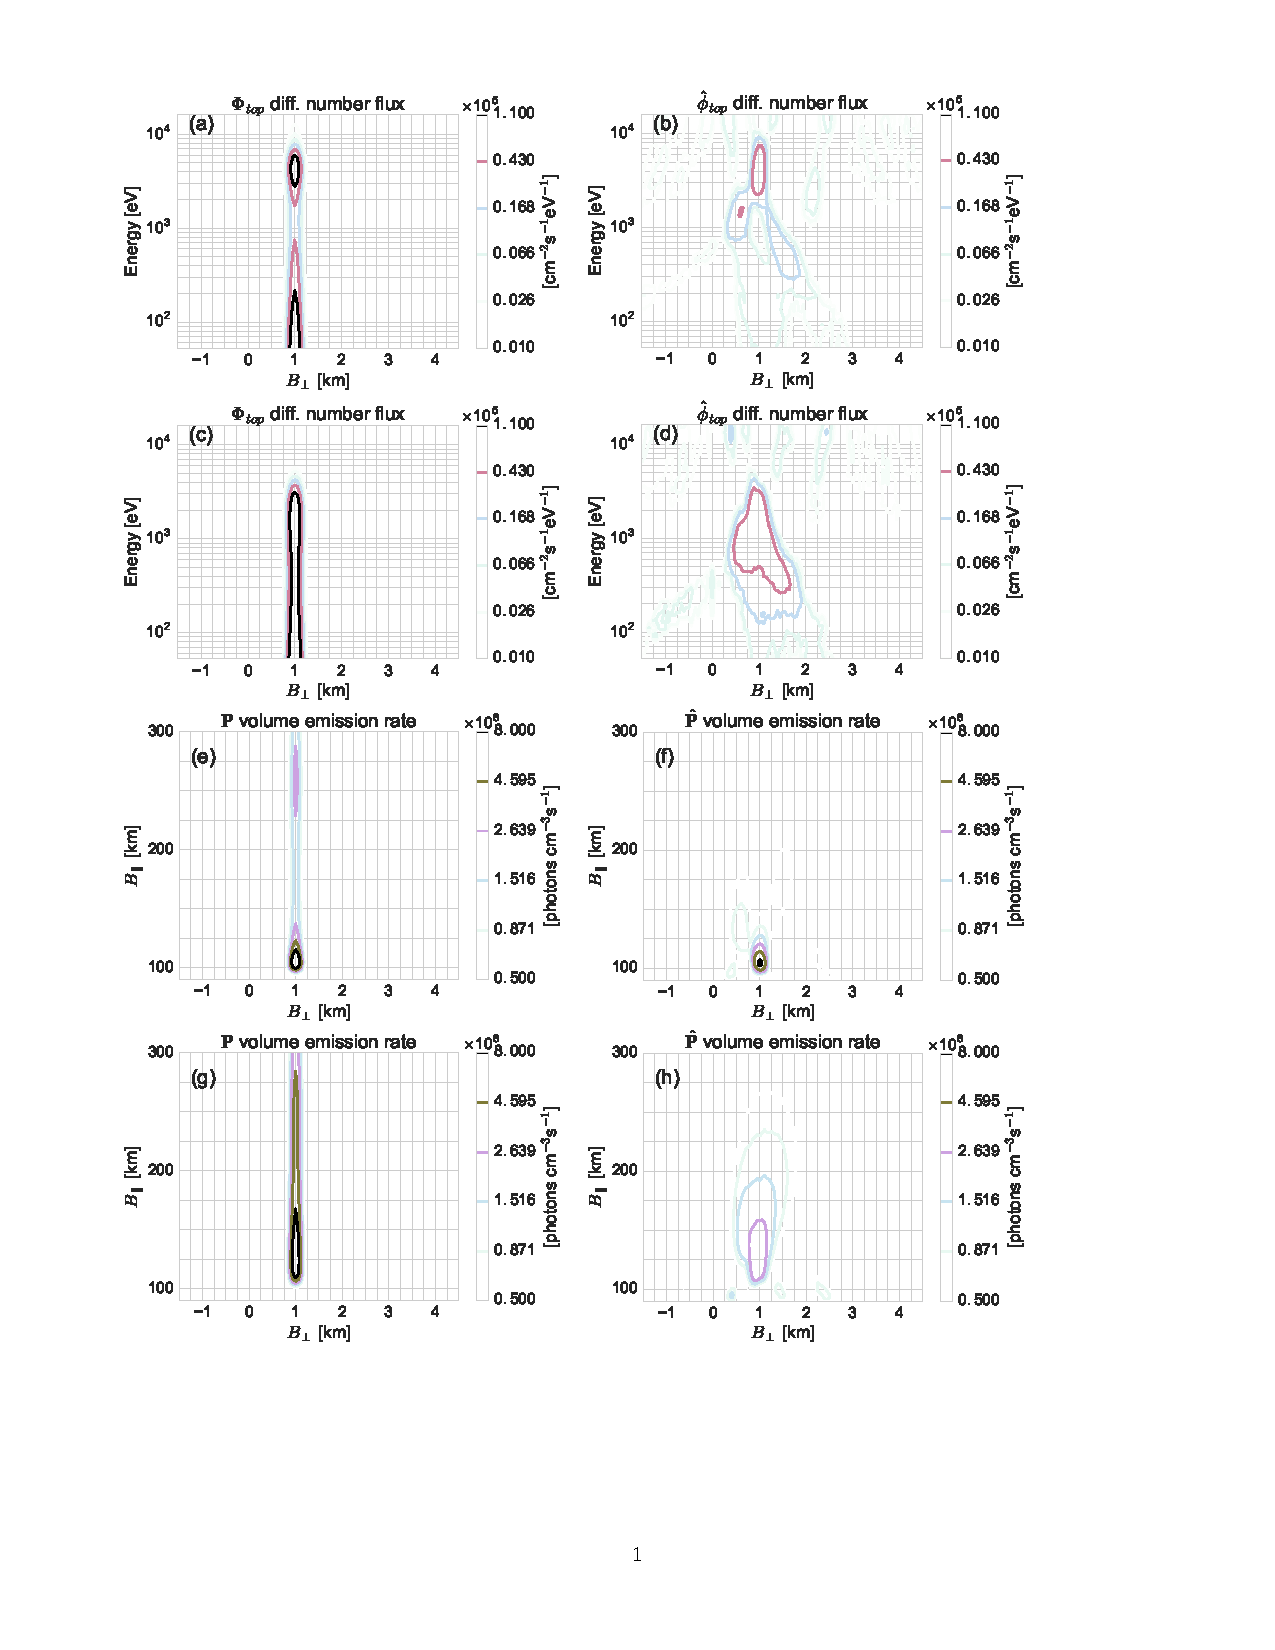
\includegraphics[trim=30 120 100 20,clip,height=0.85\textheight]{gfx/flamesim}
\caption{Flaming aurora simulation with characteristic energy $E_0\in\{4.5,1.6\}$~keV and $B_{\perp,0}=1.0$~km. 
(a)(c): differential number flux $\Phi_{top}$. (b)(d): estimated differential number flux $\hat{\Phi}_{top}$. 
(e)(g): forward modeled VER $\mathbf{P}$.  (f)(h): estimated VER $\mathbf{\hat{P}}$.} \label{fig:estflame}
\end{figure}
%
1-D cuts of $\Phi_{top}$ and $\hat{\Phi}_{top}$ at $B_{\perp}=1.0$~km are shown in Fig.~\ref{fig:est1dflame}(a)(b) respectively to aid in visualizing the characteristic energy $E_0$.
Table~\ref{tab:Jestflame} describes the $E_0$ estimation error.
%
\begin{sidewaystable}\centering
\caption{Simulated estimation error for flaming and translating auroral arcs.} \label{tab:Jestflame}
	\begin{tabular}{llllll}
		\toprule
		$B_{\perp,0}$ [km] & $E_0$ [keV] & $\hat{B}_{\perp,0}$ [km] & $\hat{E}_0$ [keV] & Error $|B_{\perp,0}-\hat{B}_\perp,0|$ [\%] & Error $|E_0-\hat{E}_0|$ [\%] \\
		\midrule
		1.0 & 4.5 & 1.0 & 4.1 & \textless 5 & \textless 10 \\
		1.0 & 1.6 & 1.0 & 1.7 & \textless 5 & \textless 10 \\
		1.55 & 5.0 & 1.55 & 4.67 & \textless 5 & \textless 10 \\
		2.5 & 4.5 & 2.5 & 4.1  & \textless 5 &  \textless 20  \\ 
		2.5 & 1.6 & 2.55 & 1.2 & \textless 5 &  \textless 25  \\ 
		3.75 & 5.0 & 3.7 & 5.7 & \textless 5 & \textless 25 \\
		4.2 & 4.5 & 4.15 & 5.6  & \textless 5 &  \textless 25  \\
		4.2 & 1.6 & 4.1 & 1.15  & \textless 5 &  \textless 30  \\
		\bottomrule
	\end{tabular}
	
\end{sidewaystable}

The estimated volume emission rate $\hat{\mathbf{P}}$ as shown in Figure~\ref{fig:estflame}(f)(h) and as 1-D cuts in Figure~\ref{fig:est1dflame}(c)(d) have morphologically similar characteristics to the forward modeled volume emission rate $\mathbf{P}$ in Figure~\ref{fig:est1dflame}(e)(g), as expected.
We observe that the estimated ground-observed intensity $\hat{\mathbf{I}}$ in Figure~\ref{fig:est1dflame}(e)(f) is within a small factor of the forward model intensity $\mathbf{I}$. 
As summarized in Table~\ref{tab:Jestflame}, $\hat{\Phi}_{top,0}$ has been estimated with $E_0$ error typically less than 30\% for simulated auroral arcs within $2.5^\circ$ of magnetic zenith.

The addition of a third camera at $B_\perp=\unit[10]{km}$ initially does not appear to make a dramatic improvement in increasing the angular range from magnetic zenith for estimating $\hat{\Phi}_{top,0}$. 
It is desirable to extend the estimate of precipitation characteristics to 3-D, which intrinsically motivates incorporating more than 2 cameras into HiST.
As observed in Table~\ref{tab:Jestflame}, the $\hat{\Phi}_{top,0}$ estimate is usable to at least $2.5^\circ$ from magnetic zenith.
It is apparent that a key limit of the $B_\perp$ range of the inversion is keeping the auroral target within the common FOV of the cameras, as is trivially expected. 


\begin{figure}\centering
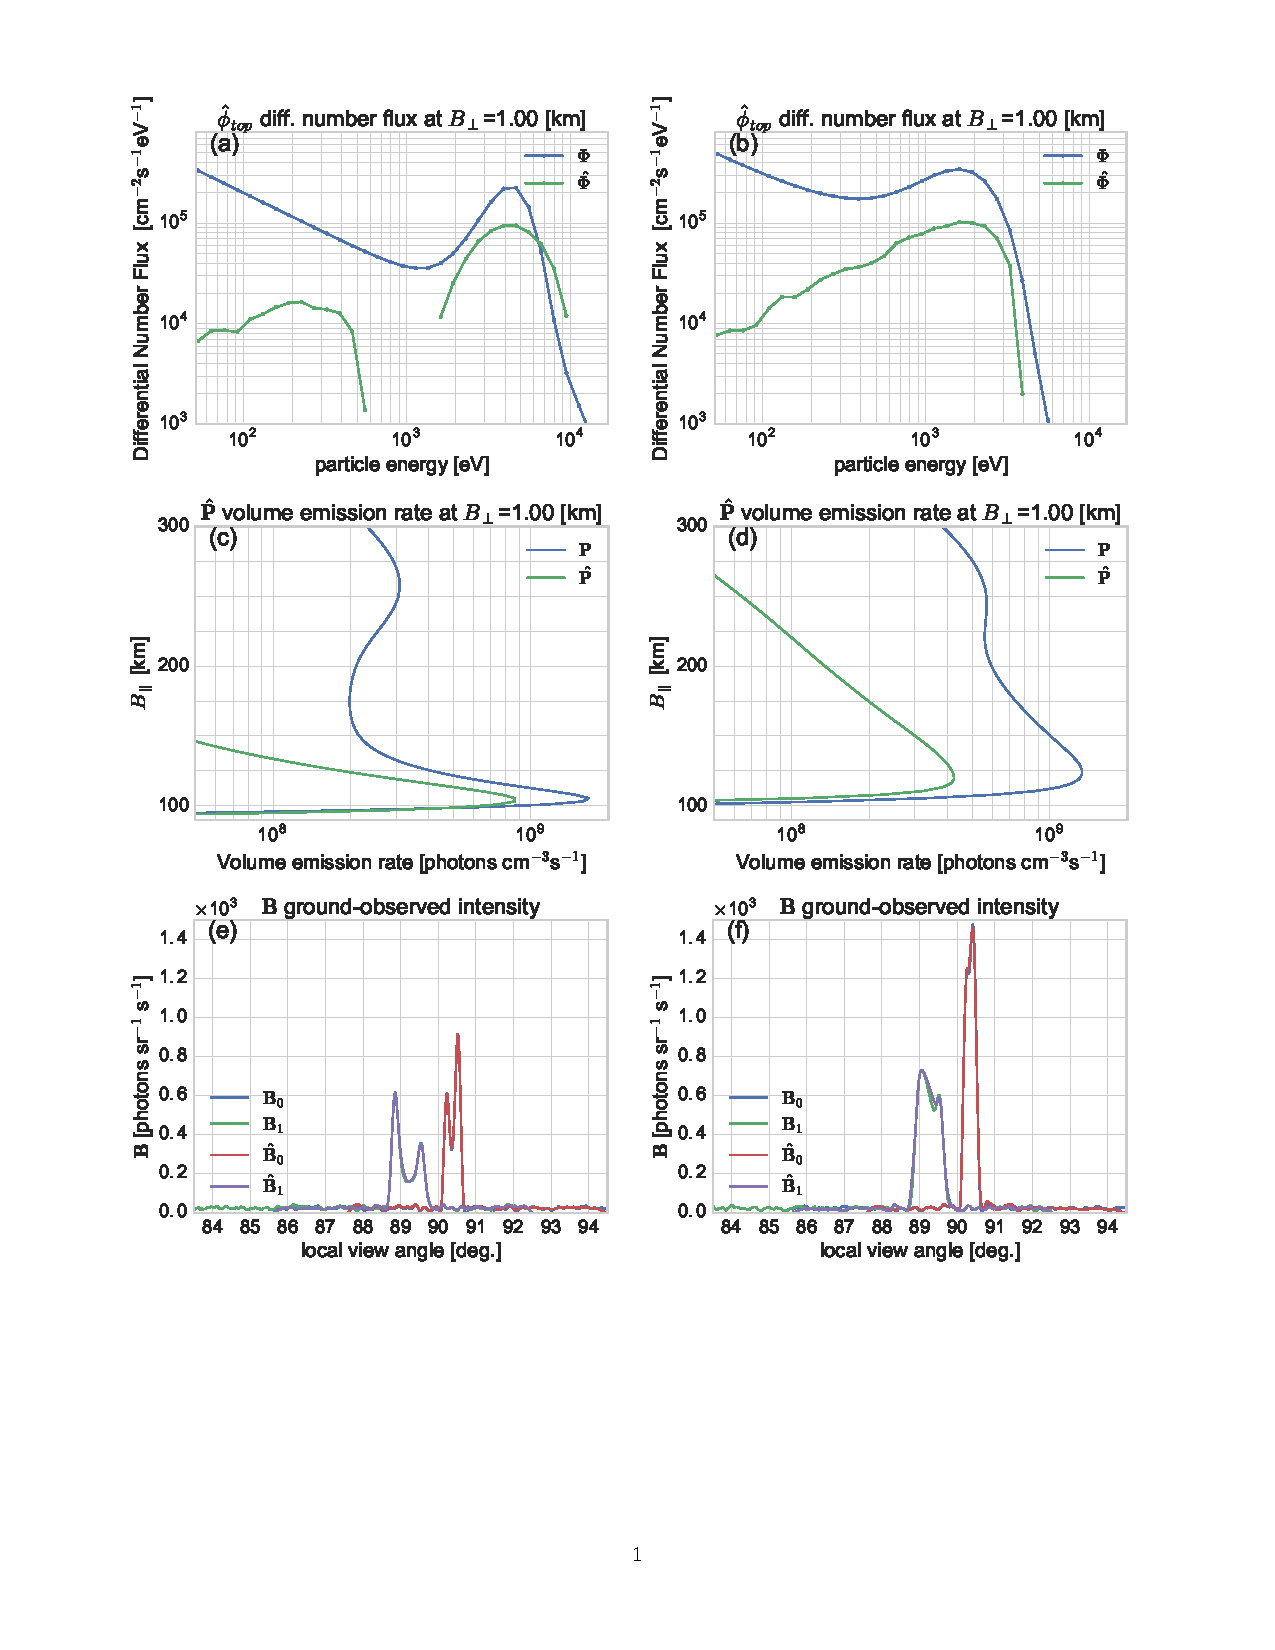
\includegraphics[trim=50 150 50 40,clip,height=0.875\textheight]{gfx/flamesim1d}
\caption{Flaming aurora simulation, 1-D cuts. 
(a)(b): Estimated differential number flux $\hat{\Phi}$.
(c)(d): Volume emission rate $\hat{\mathbf{P}}$. 
(e)(f): Ground-observed intensity $\mathbf{I}$ for characteristic energy $E_0\in\{4.5,1.6\}$~keV.}\label{fig:est1dflame}
\end{figure}
